\begin{ccRefConcept}{TriangulationDataStructure}

\ccDefinition

The \ccRefName\ concept describes objects responsible for storing and
maintaining the combinatorial part of a
$\cd$-dimensional pure simplicial complex (all simplices that are not
sub-faces of another have the same dimension $\cd$).
Its topology is the topology
of the sphere  $\sphere^\cd$ with $d\in[-2,\ad]$.
%possibly of another $\cd$-dimensional manifold without boundary 
%(that can be embedded in a higher dimension).
 In a  pure (or homogeneous) simplicial $\cd$-complex, all
 faces are sub-faces of some $\cd$-simplex. (A
simplex is also a face of itself.) In particular, it does not
contain any $\cd+1$-face, and any $\cd-1$-face belongs to exactly
two $\cd$-dimensional {full cells}. 

Values of $\cd$ (the \emph{current dimension} of the complex) include \begin{itemize}

\item[-2] This corresponds to the non-existence of any object in
the triangulation.

\item[-1] This corresponds to a single vertex and a single full cell,
  which is also the unique vertex and the unique full cell in the
  \ccc{TriangulationDataStructure}. 
 In a
geometric realization of the \ccRefName\ (\emph{e.g.}, in a
\ccc{Triangulation<TriangulationTraits, TriangulationDataStructure>} or a
\ccc{Delaunay_triangulation<DelaunayTriangulationTraits, TriangulationDataStructure>}), this vertex
corresponds to \emph{the vertex at infinity}.

\item[0] This corresponds to two vertices, each incident to one $0$-face;
the two full cells being neighbor of each other. This is the unique
triangulation of the $0$-sphere.

\item[$\cd>0$] This corresponds to a standard triangulation of the sphere
$\sphere^\cd$.
\end{itemize}

An $i$-simplex is a simplex with $i+1$ vertices. An $i$-simplex $\sigma$ is
{incident} to a $j$-simplex $\sigma'$, $j<i$, if and only if $\sigma'$
is a proper face of $\sigma$. 

We call a $0$-simplex a {\em vertex}, a $(d-1)$-simplex a {\em facet} and a
$d$-simplex a {\em full cell}. A {\em face} can have any dimension.
Two full cells are {\em adjacent} if they share a facet. Two faces are
{\em incident} if one is included un the other.


\ccHasModels

\ccc{CGAL::Triangulation_data_structure<Dimensionality, TriangulationDSVertex, TriangulationDSFullCell>}

%\ccTypes
%\ccThree{typedef std::pair<Full_cell_handle, int>}{Facet;}{}
%\ccThreeToTwo

\ccNestedType{Vertex}
{
Vertex type.
}
\ccGlue
\ccNestedType{Full_cell}
{
Full cell type.
}

The concept \ccRefName\ also defines a type for describing facets of the
triangulation with codimension~1:


%\ccThree{typedef std::pair<Full_cell_handle, int>}{Facet;}{}
%\ccTypedef{typedef std::pair<Full_cell_handle, int> Facet;}
\ccNestedType{Facet}
{
The constructor \ccc{Facet(c,i)} constructs a \ccc{Facet} representing the facet of
full cell \ccc{c} opposite to its \ccc{i}-th vertex. Its dimension is
\ccc{current_dimension()-1}.
}
\ccThreeToTwo

\ccNestedType{Face}
{A model of the concept \ccc{TriangulationDSFace}.}

Vertices and full cells are manipulated via \emph{handles}. Handles support the
usual two dereference operators \ccc{operator*} and \ccc{operator->}.

\ccNestedType{Vertex_handle}
{
Handle to a \ccc{Vertex}.
}
\ccGlue
\ccNestedType{Full_cell_handle}
{
Handle to a \ccc{Full_cell}.
}


Requirements for \ccc{Vertex} and \ccc{Full_cell} are described in concepts
\ccc{TriangulationDataStructure::Vertex} and
\ccc{TriangulationDataStructure::FullCell} \lcTex{(
\ccRefPage{TriangulationDataStructure::Vertex} and
\ccRefPage{TriangulationDataStructure::FullCell})}.

\begin{ccAdvanced}
\ccNestedType{template <typename Vb2> struct Rebind_vertex}
{This nested template class allows to get the type of a triangulation
data structure that only changes the vertex type.  It has to define a type
\ccc{Other} which is a {\it rebound} triangulation data structure, that is, the
one whose \ccc{TriangulationDSVertexBase} will be \ccc{Vb2}.}
\ccGlue
\ccNestedType{template <typename Fcb2> struct Rebind_full_cell}
{This nested template class allows to get the type of a triangulation
data structure that only changes the full cell type.  It has to define a type
\ccc{Other} which is a {\it rebound} triangulation data structure, that is, the
one whose \ccc{TriangulationDSFullCellBase} will be \ccc{Fcb2}.}
\end{ccAdvanced}


Vertices, facets and full cells can be iterated over using \emph{iterators}.
Iterators support the usual two dereference operators \ccc{operator*} and
\ccc{operator->}.

\ccNestedType{Vertex_iterator}
{
Iterator over the list of vertices.
}
\ccGlue
\ccNestedType{Full_cell_iterator}
{
Iterator over the list of full cells.
}
\ccGlue
\ccNestedType{Facet_iterator}
{
Iterator over the facets of the complex.
}

\ccNestedType{size_type}{Size type (an unsigned integral type)}
\ccGlue
\ccNestedType{difference_type}{Difference type (a signed integral type)}

\ccCreation
\ccCreationVariable{tds}

\ccConstructor{TriangulationDataStructure(int dim = 0);}{Creates an instance \ccVar\ of
type \ccRefName. The maximal dimension of its full cells is \ccc{dim} and
\ccVar\ is initialized to the empty triangulation. Thus,
\ccVar.\ccc{current_dimension()} equals \ccc{-2}.
The parameter \ccc{dim} can be ignored by the constructor if it is already
known at compile-time. Otherwise, the following precondition holds:
\ccPrecond \ccc{dim>0}.}

%\ccOperations

\ccHeading{Queries}	% --------------------------------------------- QUERIES
\ccThree{OutputIterator}{tds.number_of_full_cells() const}{}

\ccMethod{int maximal_dimension() const;} { Returns the maximal dimension of
the full dimensional cells that can be stored in the triangulation \ccVar. \ccPostcond the
returned value is positive. }

\ccMethod{int current_dimension() const;} { Returns the dimension of the
full dimensional cells stored in the triangulation. It holds that
\ccVar.\ccc{current_dimension()=-2} if and only if \ccVar.\ccc{empty()} is
\ccc{true}. \ccPostcond the returned value \ccc{d} satisfies 
$-2\leq d \leq$\ccVar.\ccc{maximal_dimension()}. }

\ccMethod{bool empty() const;} { Returns \ccc{true} if thetriangulation
contains nothing. Returns \ccc{false} otherwise. }

\ccMethod{size_type number_of_vertices() const;}
{Returns the number of vertices in the triangulation.}

\ccMethod{size_type number_of_full_cells() const;}
{Returns the number of full cells  in the triangulation.}

\ccMethod{bool is_vertex(const Vertex_handle & v) const;}
{Tests whether \ccc{v} is a vertex of the triangulation. }

\ccMethod{bool is_full_cell(const Full_cell_handle & c) const;}
{Tests whether \ccc{c} is a full cell of the triangulation.}

\ccMethod{template< typename TraversalPredicate, typename OutputIterator >
void full_cells(Full_cell_handle c, TraversalPredicate & tp,
OutputIterator & out) const;}
{This function computes (\emph{gathers}) a connected set of full cells
satifying a common criterion. Call them \emph{good} full cells. It is assumed
that the argument \ccc{c} is a good full cell. The full cells are then
recursively explored by examining if, from a given good full cell, its adjacent
full cells are also good.\\
The argument \ccc{tp} is a predicate that takes as argument a \ccc{Facet}
whose defining \ccc{Full_cell} is good. The predicate must return \ccc{true}
if the traversal of that \ccc{Facet} leads to a good full cell.\\
All the good full cells are output into the last argument \ccc{out}.
\ccPrecond \ccc{c!=Full_cell_handle()} and \ccc{tp(c)==true}.
}

\ccMethod{template< typename OutputIterator > OutputIterator
incident_full_cells(Vertex_handle v, OutputIterator out) const;}
{Insert in \ccc{out} all the full cells that are incident to the vertex
\ccc{v}, {i.e.}, the full cells that have the \ccc{Vertex v} as a vertex.
Returns the output iterator.
\ccPrecond \ccc{v!=Vertex_handle()}.
}

\ccMethod{template< typename OutputIterator > OutputIterator
incident_full_cells(const Face & f, OutputIterator out) const;}
{Insert in \ccc{out} all the full cells that are incident to the face \ccc{f},
{i.e.}, the full cells that have the \ccc{Face f} as a subface.
Returns the output iterator.
\ccPrecond\ccc{f.full_cell()!=Full_cell_handle()}.
}

\ccMethod{template< typename OutputIterator > OutputIterator
star(const Face & f, OutputIterator out) const;}
{Insert in \ccc{out} all the full cells that share at least one vertex with the \ccc{Face
f}. Returns the output iterator.
%\ccPrecond\ccc{f.full_cell()!=Full_cell_handle()}.
}

\ccMethod{template< typename OutputIterator > OutputIterator
 incident_faces(Vertex_handle v, const int d, OutputIterator
 out);}{Constructs all the \ccc{Face}s of dimension \ccc{d} incident to
 \ccc{Vertex} v and inserts them in the \ccc{OutputIterator out}.  If \ccc{d
 >=} \ccVar.\ccc{current_dimension()}, then no \ccc{Face} is
 constructed.
\ccPrecond\ccc{0 < d} and \ccc{v!=Vertex_handle()}.
}


%%%%%%%%%%%%%%%%%%%%%%%%%%%%%%%%%%%%%%%%%%%%%%%%%%%%%%%
%    Since unused from the moment and usage is not clear, I remove it
%    for the moment.
%%%%%%%%%%%%%%%%%%%%%%%%%%%%%%%%%%%%%%%%%%%%%%%%%%%%%%%
% \ccMethod{template< typename OutputIterator > OutputIterator
% incident_upper_faces(Vertex_handle v, const int d, OutputIterator
%  out);}{Constructs all the {\em upper} \ccc{Face}s of dimension \ccc{d}
%  incident to \ccc{Vertex} v and inserts them in the \ccc{OutputIterator out}.\\
%  Assuming some total ordering on the vertices of the complex (which is
%  invariant as long as no vertex is inserted in or removed from the complex), a
%  \ccc{Face} incident to \ccc{v} is an {\em upper} \ccc{Face} if and only if
%  its vertices occur at \ccc{v} or beyond \ccc{v} in the ordering.\\ In
%  particular, taking the disjoint union of the upper \ccc{Face}s of dimension
%  \ccc{d} incident to every vertex of the complex yields exactly the set of
%  faces of dimension \ccc{d} of the complex.\\ The constructed \ccc{Faces} are
%  lexicographically ordered (using the vertex order as base
%  ordering). If
% $d\geq$\ccVar.\ccc{current_dimension()}, then no \ccc{Face} is
%  constructed.
% \ccPrecond\ccc{0 < d} and \ccc{v!=Vertex_handle()}.
% }

% \ccGlue\ccMethod{template< typename OutputIterator, typename Comparator >
%  OutputIterator incident_upper_faces(Vertex_handle v, const int d,
%  OutputIterator out, Comparator cmp);} {Same as above, but uses \ccc{cmp} as
%  the vertex ordering to define the upper faces.}

\ccHeading{Accessing the vertices} % --------------------- ACCESS TO VERTICES
\ccThree{Vertex_iterator}{tds.number_of_full_cells() const}{}

\ccMethod{Vertex_handle vertex(Full_cell_handle c, const int i) const;}%{}
{ Returns a handle to the \ccc{i}-th \ccc{Vertex} of the \ccc{Full_cell} \ccc{c}.
\ccPrecond $0\leq i\leq$\ccVar.\ccc{current_dimension()} and \ccc{c!=Full_cell_handle()}.}

\ccMethod{int mirror_index(Full_cell_handle c, int i) const;}%{}
{Returns the index of the vertex mirror of the \ccc{i}-th vertex of \ccc{c}.
Equivalently, returns the index of \ccc{c} as a neighbor of  its \ccc{i}-th neighbor.
\ccPrecond $0\leq i\leq$\ccVar.\ccc{current_dimension}()\\
and \ccc{c!=Full_cell_handle()}. }

\ccMethod{Vertex_handle mirror_vertex(Full_cell_handle c, int i) const;}%{}
{Returns the vertex mirror of the \ccc{i}-th vertex of \ccc{c}.
Equivalently, returns the vertex of the \ccc{i}-th neighbor of \ccc{c}
that is not vertex of \ccc{c}.
\ccPrecond $0\leq i\leq$\ccVar.\ccc{current_dimension}()\\
and \ccc{c!=Full_cell_handle()}. }


\ccMethod{Vertex_iterator vertices_begin();}
{
The first vertex of \ccVar. User has no control on the order.
}
\ccGlue
\ccMethod{Vertex_iterator vertices_end();}
{
The beyond vertex of \ccVar.
}

\ccHeading{Accessing the full cells} % ------------------- ACCESS TO CELLS
\ccThree{Full_cell_iterator}{tds.number_of_full_cells() const}{}

\ccMethod{Full_cell_handle full_cell(Vertex_handle v) const;}%{}
{Returns a full cell incident to \ccc{Vertex} \ccc{v}. Note that this
  full cell is
not unique (\ccc{v} is typically incident to more than one full cell).
\ccPrecond\ccc{v} is not the default constructed \ccc{Vertex_handle}}

\ccMethod{Full_cell_handle neighbor(Full_cell_handle c, int i) const;}%{}
{ Returns a \ccc{Full_cell_handle} pointing to the \ccc{Full_cell}
opposite to the \ccc{i}-th vertex of \ccc{c}. 
\ccPrecond$0\leq i \leq$\ccVar.\ccc{current_dimension()}\\
and \ccc{c} is not the default constructed \ccc{Full_cell_handle}}

\ccMethod{Full_cell_iterator full_cells_begin();}
{
The first full cell of \ccVar.  User has no control on the order.
}
\ccGlue
\ccMethod{Full_cell_iterator full_cells_end();}
{
The beyond full cell of \ccVar.
}

\ccHeading{Faces and Facets} % - - - - - - - - - - - - - - - - - - - - FACETS

\ccMethod{Facet_iterator facets_begin();}
{Iterator to the first facet of the triangulation.}
\ccGlue
\ccMethod{Facet_iterator facets_end();}
{Iterator to the beyond facet of the triangulation.}

\ccMethod{Full_cell_handle full_cell(const Facet & f) const;}
{Returns a full cell containing the facet \ccc{f}}

\ccMethod{int index_of_covertex(const Facet & f) const;}
{Returns the index of vertex of the full cell \ccc{c=}\ccVar.\ccc{full_cell(f)}
which does {not} belong to \ccc{c}.}

%\begin{ccAdvanced}
%
%\ccMethod{bool is_boundary_facet(const Facet & f) const;}
%{When a subset of the full cells has their \ccc{flags} set to \ccc{1}, this
%function returns \ccc{true} when the \ccc{Facet f} is part of the boundary of
%that subset, and \ccc{false} otherwise.
%\note{OD: bof, ces trucs de flags sont publics ? si oui ils faut qu'ils
%  soient robustes et documente partout}
%\note{SH: Oui, a mon avis, il faut virer cette fonction de la doc.}
%}
%
%\end{ccAdvanced}


\ccHeading{Vertex insertion} % - - - - - - - - - - - - - - - - - - INSERTIONS

\ccMethod{Vertex_handle insert_in_full_cell(Full_cell_handle c);}
{Inserts a new
vertex \ccc{v} in the full cell \ccc{c} and returns a handle to
it. The full cell
\ccc{c} is subdivided into \ccVar.\ccc{current_dimension()}+1 full cells which
share the vertex \ccc{v} (see Figure~\ref{triangulation:fig:insert-full-cell}).
\ccPrecond Current dimension is positive and \ccc{c} is a full cell of
\ccVar.}

\begin{figure}[ht]
\begin{ccTexOnly}
\begin{center}
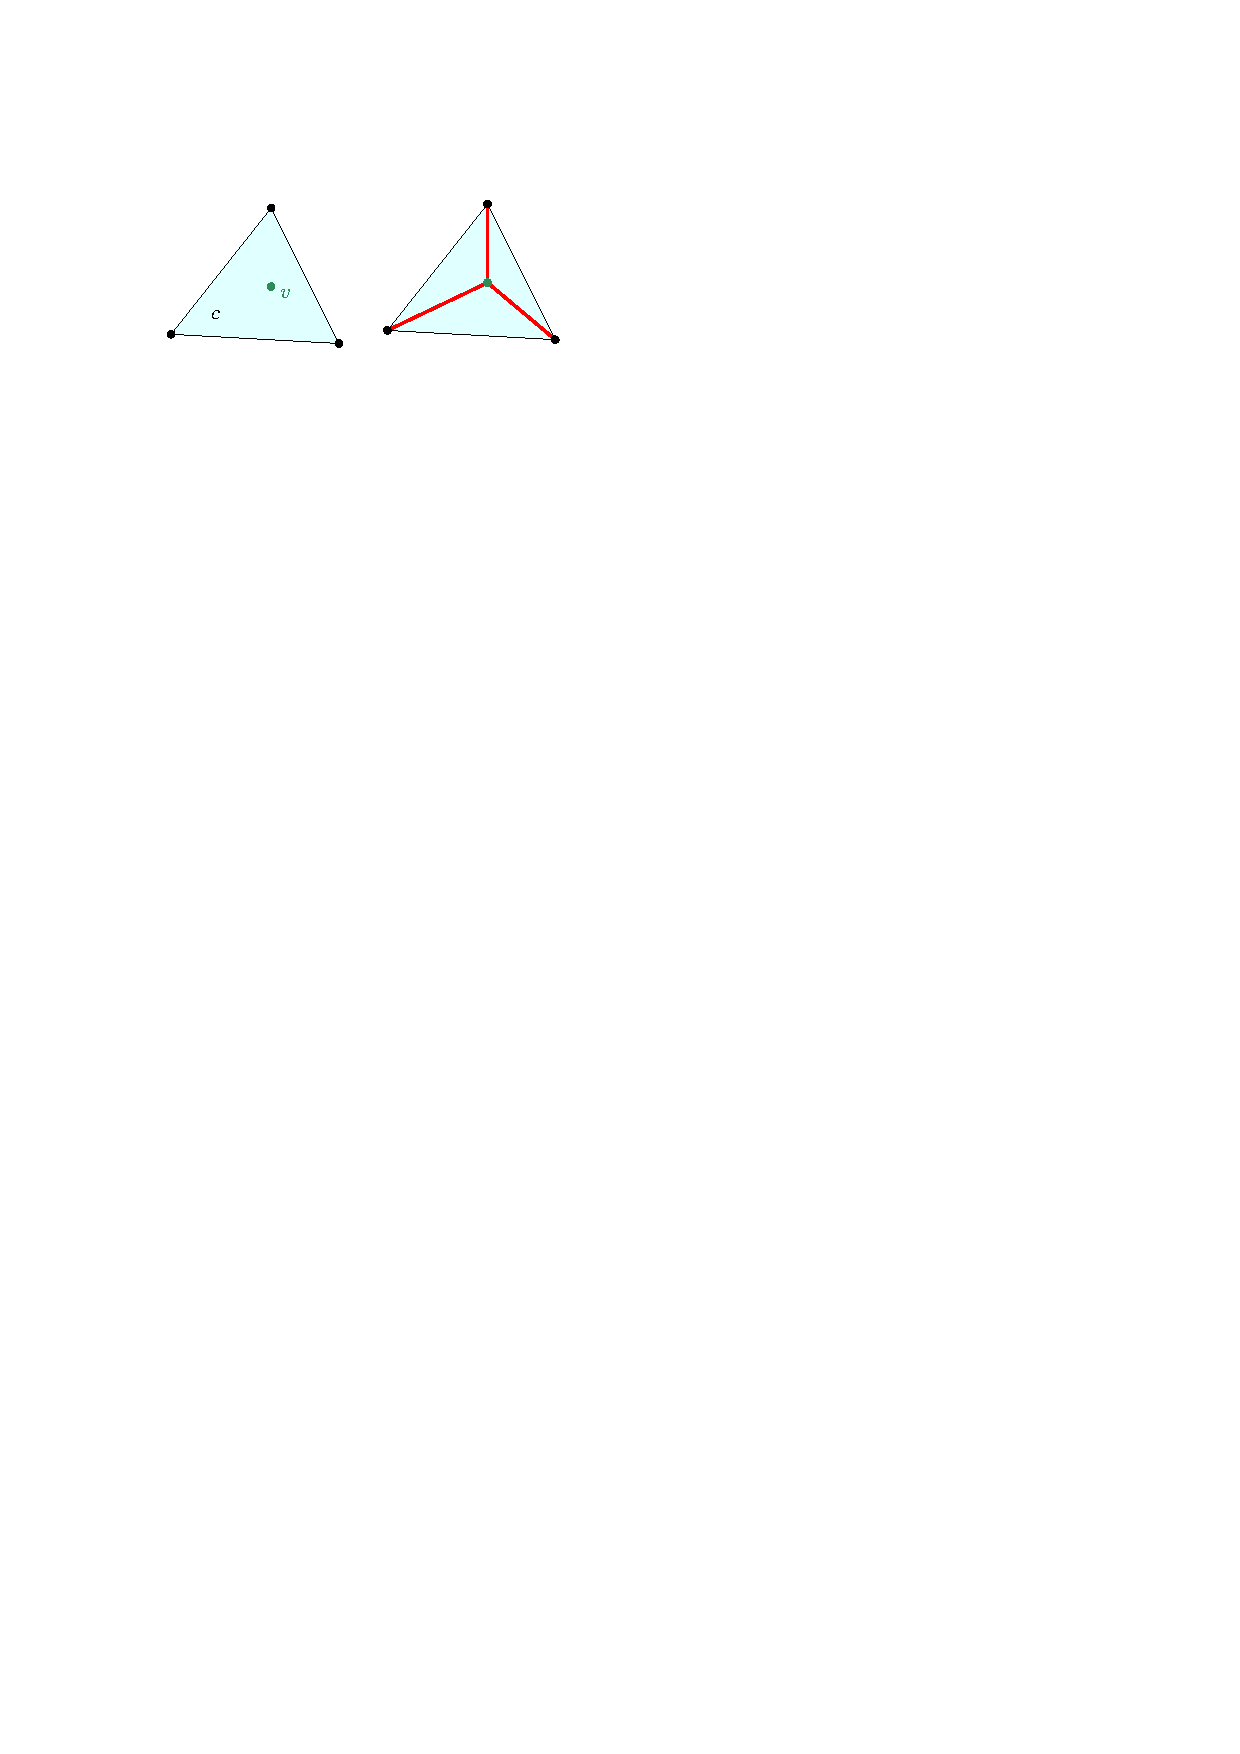
\includegraphics{Triangulation_ref/fig/insert-in-cell.pdf}
\end{center}
\end{ccTexOnly}
\begin{ccHtmlOnly}
<center>
<img border=0 src="./fig/insert-in-cell.png" align="middle" alt="The effect of insert_in_full_cell()">
</center>
\end{ccHtmlOnly}
\caption{Insertion in a full cell, $\cd=2$\label{triangulation:fig:insert-full-cell}}
\end{figure}

\ccMethod{Vertex_handle insert_in_face(const Face & f);}
{Inserts a vertex in the triangulation data structure by subdividing the
\ccc{Face f}. Returns a handle to the newly created \ccc{Vertex} (see
Figure below~\ref{triangulation:fig:insert-face}).}

\begin{figure}[ht]
\begin{ccTexOnly}
\begin{center}
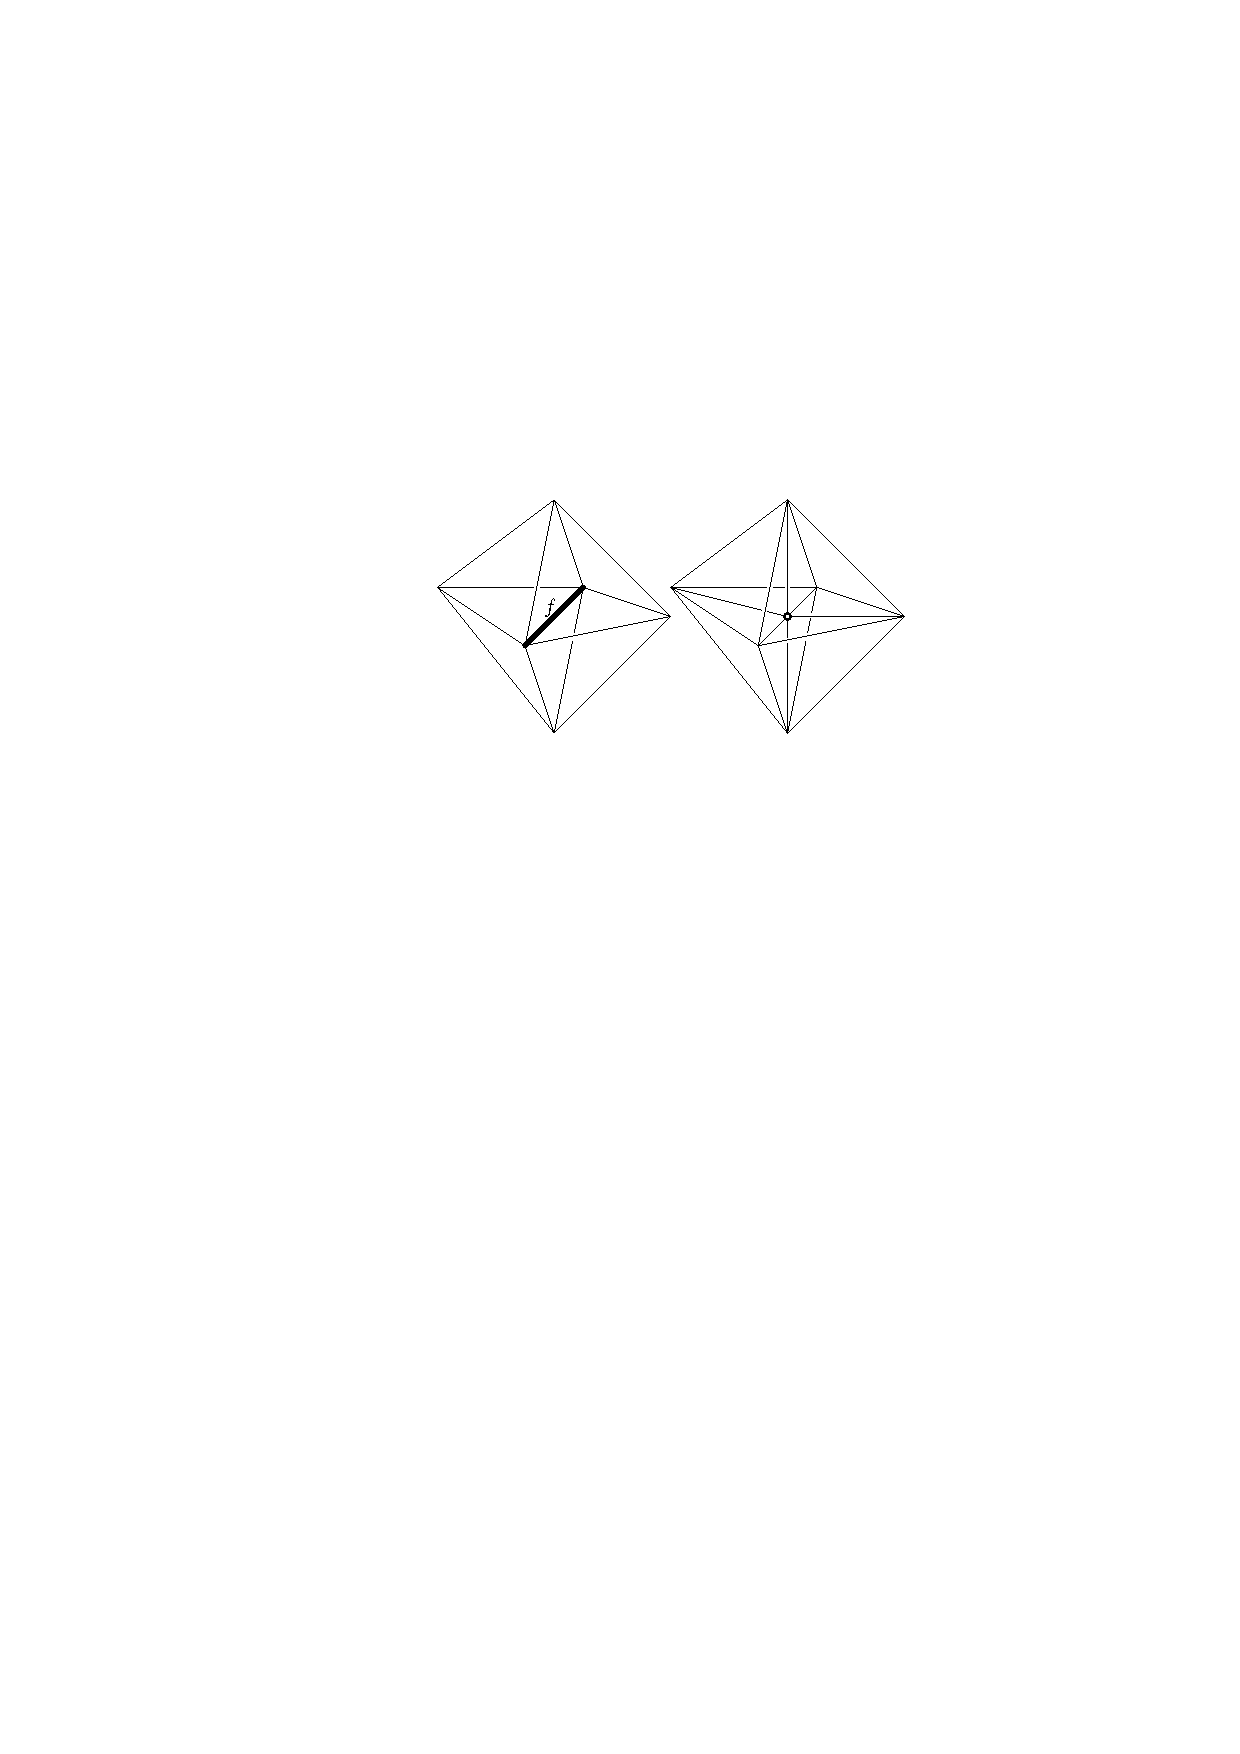
\includegraphics{Triangulation_ref/fig/insert-in-face.pdf}
\end{center}
\end{ccTexOnly}
\begin{ccHtmlOnly}
<center>
<img border=0 src="./fig/insert-in-face.png" align="middle" alt="The effect of insert_in_face()">
</center>
\end{ccHtmlOnly}
\caption{Insertion in face, $\cd=3$\label{triangulation:fig:insert-face}}
\end{figure}

\ccMethod{Vertex_handle insert_in_facet(const Facet & ft);}
{Inserts a vertex in the triangulation data structure by subdividing the
\ccc{Facet ft}. Returns a handle to the newly created \ccc{Vertex}.}



\ccMethod{template< class ForwardIterator > Vertex_handle
insert_in_hole(ForwardIterator start, ForwardIterator end, Facet f);}{The
full cells in the range $C=$\ccc{[start, end)} are removed, thus
forming a hole $H$.
A \ccc{Vertex} is inserted and connected to the boundary of the hole in order
to ``fill it''. A \ccc{Vertex_handle} to the new \ccc{Vertex} is returned
(see Figure~\ref{triangulation:fig:insert-hole}).
\ccPrecond 
\ccc{c} belongs to $C$ and \ccc{c->neighbor(i)}
does not,  with \ccc{f=(c,i)}.
$H$ the union of full cells in $C$ is simply connected and its
boundary $\partial H$ is a
combinatorial triangulation of the sphere $\sphere^{d-1}$.
All vertices of the triangulation are on  $\partial H$.
}
\ccGlue
\ccMethod{template< class ForwardIterator, class OutputIterator >
Vertex_handle insert_in_hole(ForwardIterator start, ForwardIterator end, Facet
f, OutputIterator out);}{Same as above, but handles to the new full cells are
appended to the \ccc{out} output iterator.}

\begin{figure}[ht]
\begin{ccTexOnly}
\begin{center}
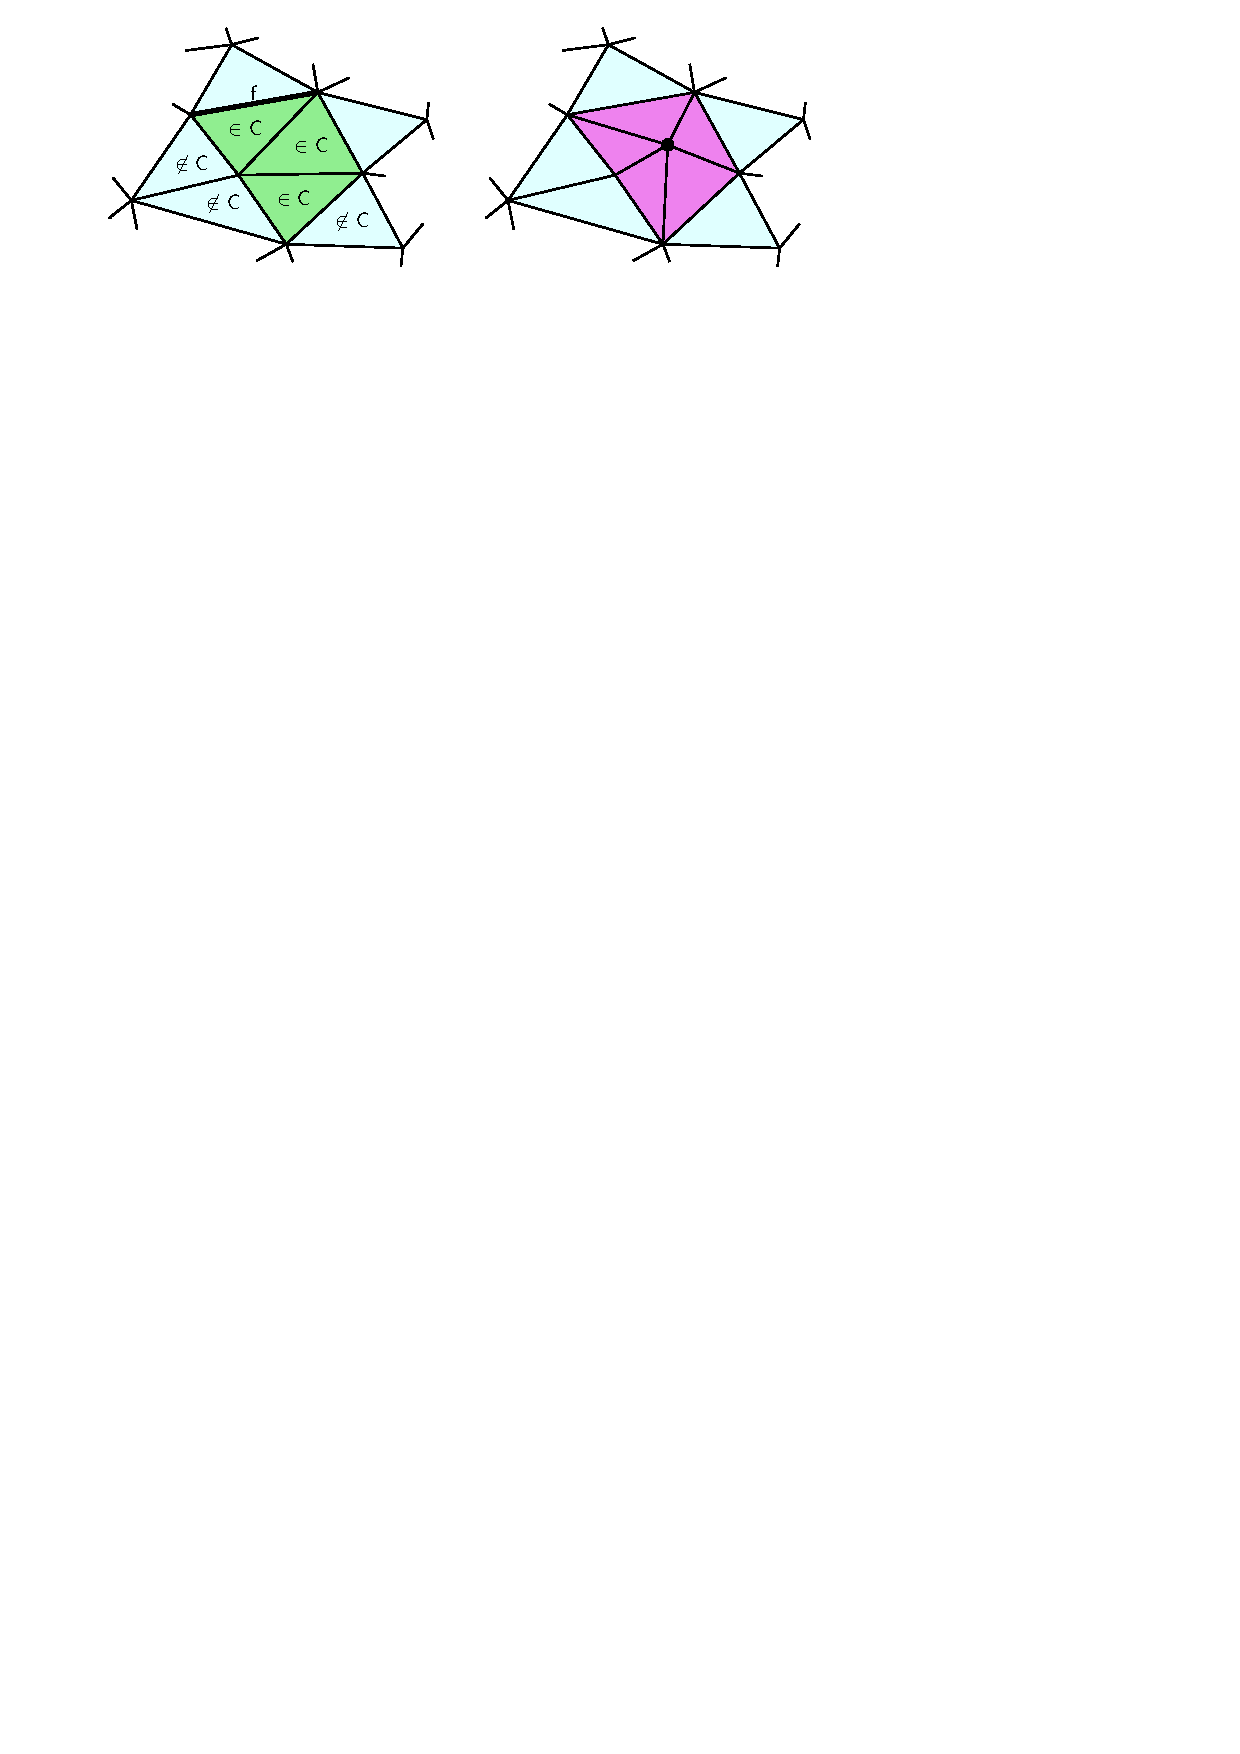
\includegraphics{Triangulation_ref/fig/insert-in-hole.pdf}
\end{center}
\end{ccTexOnly}
\begin{ccHtmlOnly}
<center>
<img border=0 src="./fig/insert-in-hole.png" align="middle" alt="The effect of insert_in_hole()">
</center>
\end{ccHtmlOnly}
\caption{Insertion in a hole, $\cd=2$\label{triangulation:fig:insert-hole}}
\end{figure}

\ccMethod{Vertex_handle insert_increase_dimension(Vertex_handle star);}
{Transforms a triangulation of  the sphere $\sphere^d$ into the
triangulation of the sphere $\sphere^{d+1}$ by adding a new vertex
\ccc{v}.
\ccc{v} is used to triangulate one of the two half-spheres of
$\sphere^{d+1}$ ($v$ is added as $(d+2)^{th}$ vertex to all
full cells)
and \ccc{star} is used to triangulate the other half-sphere
(all full cells that do not already have star as vertex are duplicated,
and \ccc{star} replaces \ccc{v} in these full cells).
The indexing of the vertices in the
full cell is such that, if \ccc{f} was a full cell of maximal dimension in the
initial complex, then \ccc{(f,v)}, in this order, is the corresponding full cell
in the updated triangulation. A handle to \ccc{v} is returned
(see Figure~\ref{triangulation:fig:insert-increase-dim}).
\ccPrecond\ccVar.
If the current dimension is -2 (empty triangulation), then \ccc{star}
has to be omitted, otherwise
the current dimension must be strictly less than the maximal dimension
and \ccc{star} must be a vertex of \ccVar.}

\begin{figure}[ht]
\begin{ccTexOnly}
\begin{center}
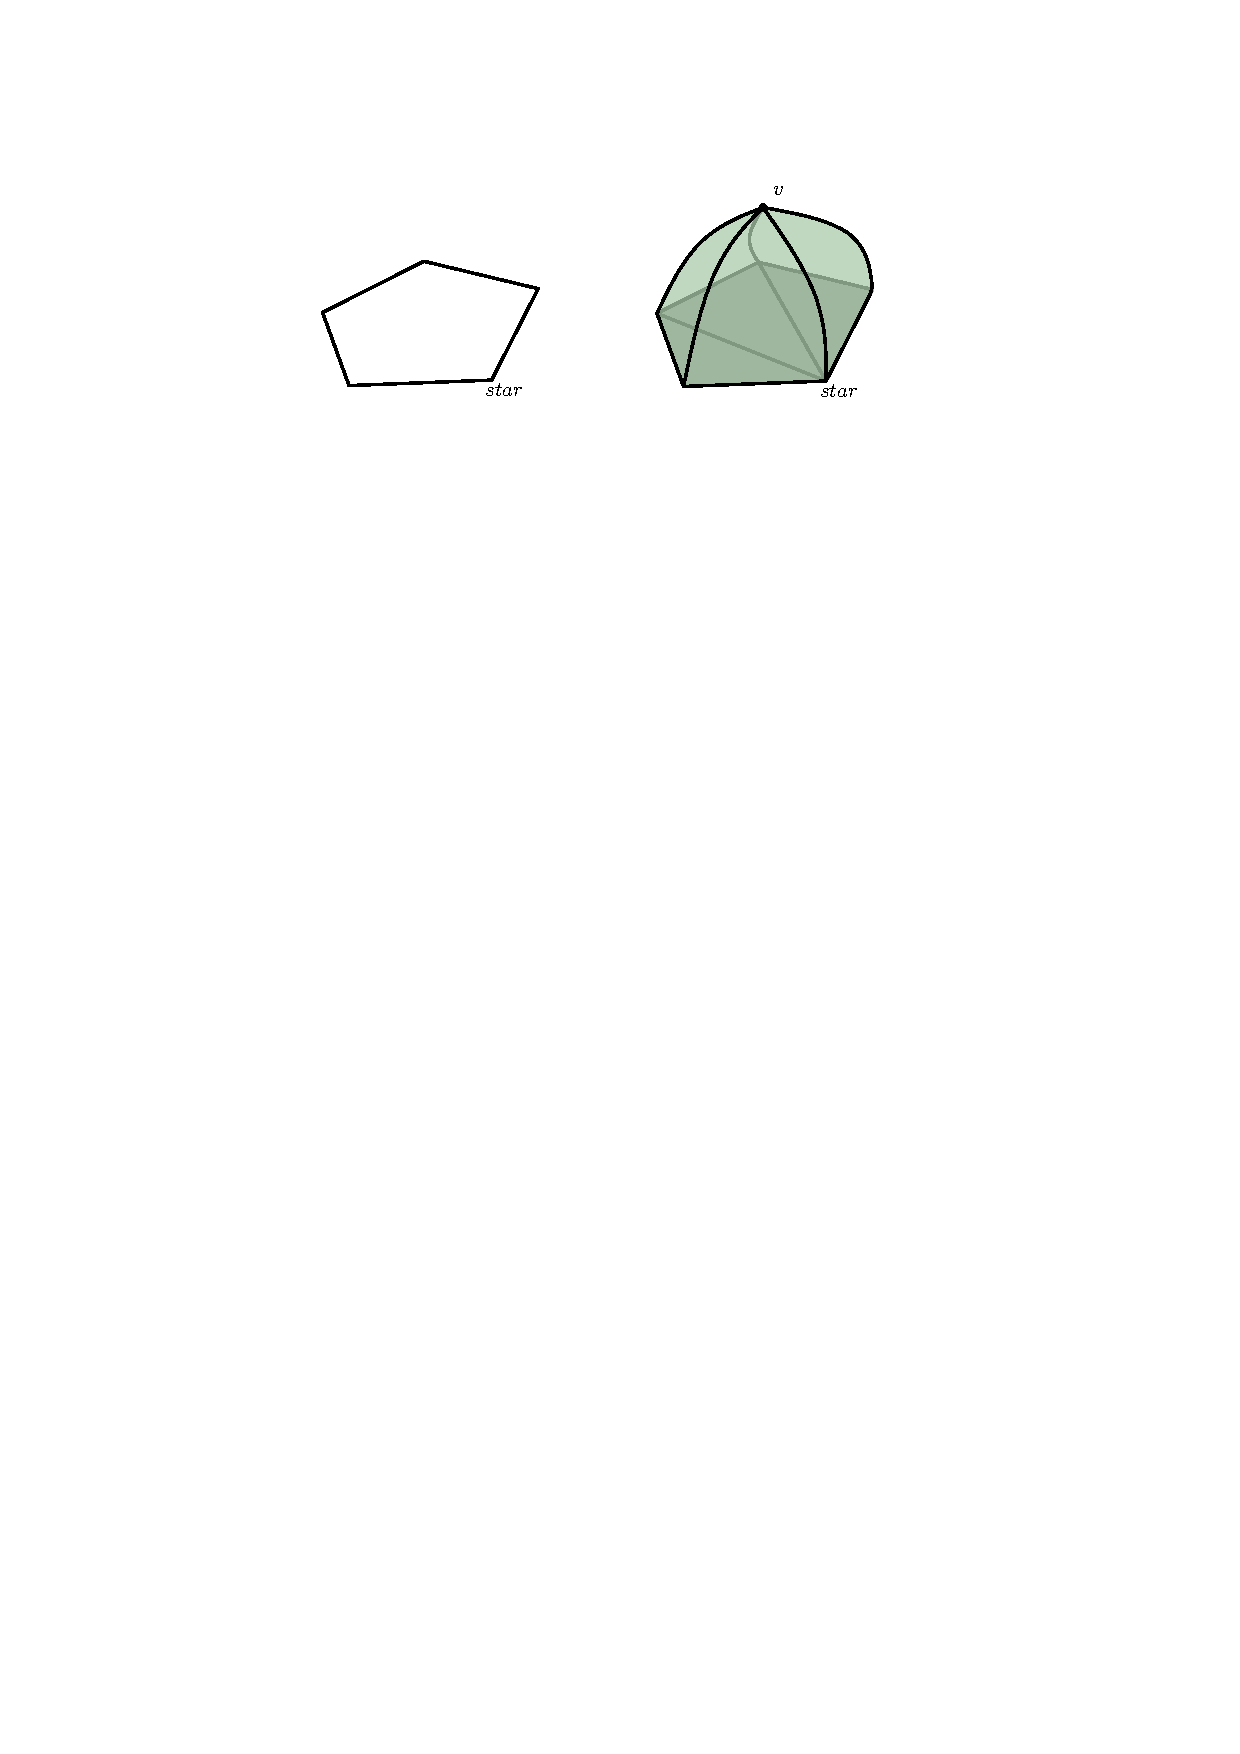
\includegraphics{Triangulation_ref/fig/insert-increase-dim.pdf}
\end{center}
\end{ccTexOnly}
\begin{ccHtmlOnly}
<center>
<img border=0 src="./fig/insert-increase-dim.png" align="middle" alt="The effect of insert_increase_dimension()">
</center>
\end{ccHtmlOnly}
\caption{Insertion, increasing the dimension from $\cd=1$ to $\cd=2$\label{triangulation:fig:insert-increase-dim}}
\end{figure}

\begin{ccAdvanced}


\ccMethod{Full_cell_handle new_full_cell();} {Adds a new full cell to \ccVar\ and
returns a handle to it. The new full cell has no vertex and no neighbor yet.}

\ccMethod{Vertex_handle new_vertex();}
{Adds a new vertex to \ccVar\ and returns a handle to it. The new vertex has
no associated full cell nor index yet.}

\ccMethod{void associate_vertex_with_full_cell(Full_cell_handle c, int i,
Vertex_handle v);}
{Sets the \ccc{i}-th vertex of \ccc{c} to \ccc{v} and, if \ccc{v} is non-NULL,
sets \ccc{c} as the incident full cell of \ccc{v}.}

\ccMethod{void set_neighbors(Full_cell_handle ci, int i, Full_cell_handle cj, int
j);}
{Sets the neighbor opposite to vertex \ccc{i} of \ccc{Full_cell} \ccc{ci} to
\ccc{cj}. Sets the neighbor opposite to vertex \ccc{j} of \ccc{Full_cell}
\ccc{cj} to \ccc{ci}.}

\ccMethod{void set_current_dimension(int d);} { Forces the current dimension
of the complex to \ccc{d}. 
\ccPrecond $-1\leq d\leq$\ccc{maximal_dimension()}.}

\end{ccAdvanced}

\ccHeading{Vertex removal} % - - - - - - - - - - - - - - - - - - - - REMOVALS

\ccMethod{void clear();}
{Reinitializes \ccVar\ to the empty complex.}

\ccMethod{Vertex_handle collapse_face(const Face & f);} {Contracts the
\ccc{Face f} to a single vertex. Returns a handle to that vertex
(see Figure~\ref{triangulation:fig:collapse-face}).
\ccPrecond
The boundary of the full cells incident to \ccc{f}
is a topological sphere of dimension
\ccVar.\ccc{current_dimension()}-1).
}

\begin{figure}[ht]
\begin{ccTexOnly}
\begin{center}
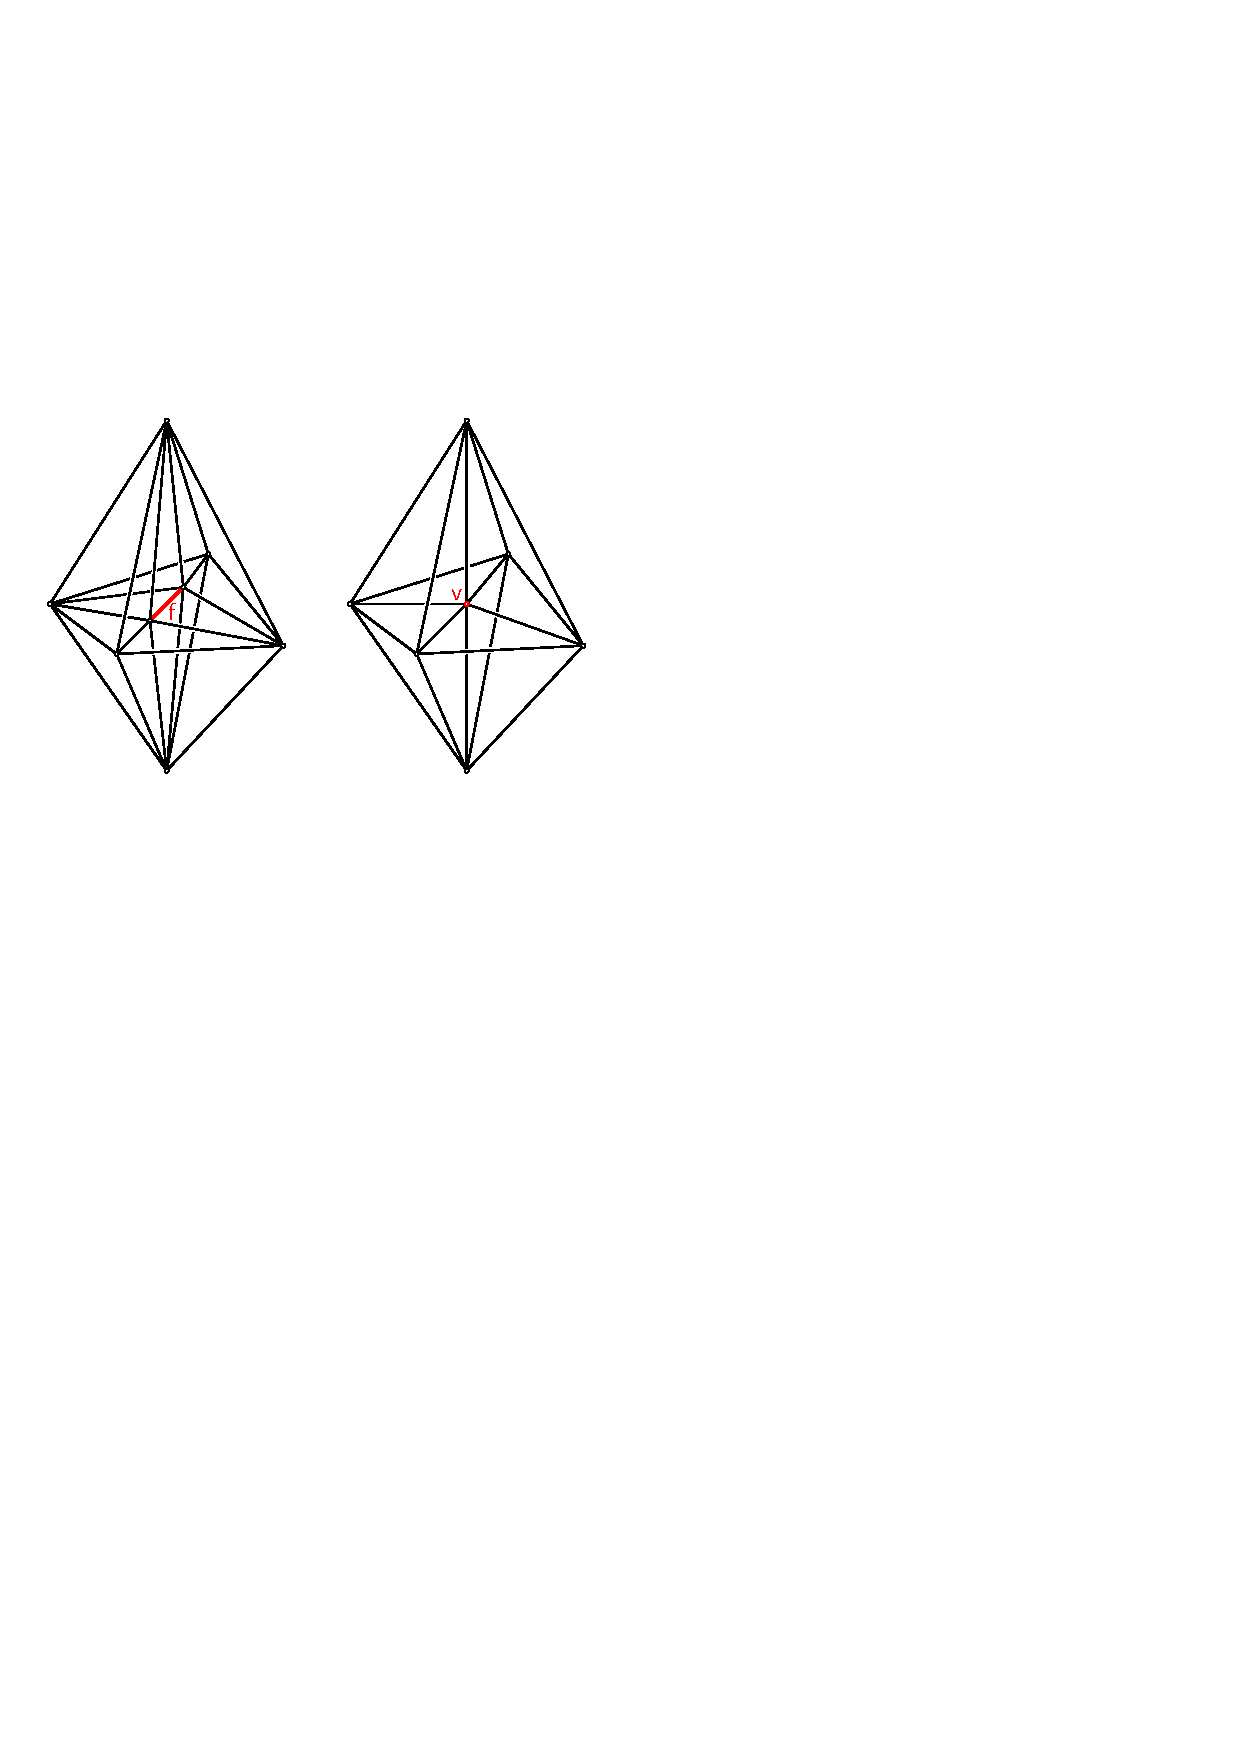
\includegraphics{Triangulation_ref/fig/collapse-face.pdf}
\end{center}
\end{ccTexOnly}
\begin{ccHtmlOnly}
<center>
<img border=0 src="./fig/collapse-face.png" align="middle" alt="The effect of collapse_face()">
</center>
\end{ccHtmlOnly}
\caption{Collapsing an edge in dimension $\cd=3$, \ccc{v} is returned\label{triangulation:fig:collapse-face}}
\end{figure}

\ccMethod{void remove_decrease_dimension(Vertex_handle v, Vertex_handle
star);} {This method does exactly the opposite of
\ccc{insert_increase_dimension()}:
\ccc{v} is removed,
full cells not containing \ccc{star} are removed
full cells containing \ccc{star} but not \ccc{v} loose vertex \ccc{star}
full cells containing \ccc{star} and \ccc{v} loose vertex \ccc{v}
(see Figure~\ref{triangulation:fig:insert-increase-dim}).
\ccPrecond 
All cells contains either \ccc{star} or \ccc{v}.
Edge \ccc{star-v} exists in the triangulation
and \ccc{current_dimension()!=2}.
}

\begin{ccAdvanced}

\ccMethod{void delete_vertex(Vertex_handle v);}
{Remove the vertex \ccc{v} from the triangulation. 
%This does not take care of
%erasing the references to \ccc{v} in other parts of the triangulation.
}

\ccMethod{void delete_full_cell(Full_cell_handle c);}
{Remove the full cell \ccc{c} from the triangulation. 
%This does not take care of
%erasing the references to \ccc{c} in other parts of the triangulation.
}

\ccMethod{template< typename ForwardIterator > void
    delete_full_cells(ForwardIterator start, ForwardIterator end);}
{Remove the full cells in the range \ccc{[start,end)} from the triangulation.
%This does not take care of erasing the references to these full cells in other parts of
%the triangulation.
}

\end{ccAdvanced}



\begin{ccDebug}
\ccHeading{Validity check} % - - - - - - - - - - - - - - - - - - - - VALIDITY

\ccMethod{bool is_valid(bool verbose=false) const;}{%
Partially checks whether \ccVar\ is indeed a triangulation.

It must \emph{at least}\begin{itemize}
\item check the validity of the vertices and full cells of \ccVar\ by calling
their respective \ccc{is_valid} method.
\item check that each full cell has no duplicate vertices and has as many
neighbors as its number of facets (\ccc{current_dimension()+1}).
\item check that each full cell share exactly \ccVar.\ccc{current_dimension()}
vertices with each of its neighbor.
\end{itemize}

Returns \ccc{true} if all the tests pass, \ccc{false} if any test fails. See
the documentation for the models of this concept to see the additionnal (if
any) validity checks that they implement.%
}

\end{ccDebug}


\ccHeading{Input/Output} % ---------------------------- I/O

\ccFunction{istream & operator>>(istream & is, TriangulationDataStructure &
tds);}
{Reads a combinatorial triangulation from \ccc{is} and assigns it to
\ccc{tds}. \ccPrecond The dimension of the input complex must be less than or
equal to \ccVar.\ccc{maximal_dimension()}.}

\ccFunction{ostream & operator<<(ostream & os, const TriangulationDataStructure
& tds);}
{Writes \ccc{tds} into the output stream \ccc{os}}

The information stored in the \ccc{iostream} is:
\\- the current dimension (which must be \ccc{<=}\ccVar.\ccc{maximal_dimension()}), 
\\- the number of vertices,
\\- for each vertex the information of that vertex,
\\- the number of full cells, 
\\- for each full cell the indices of its vertices and extra information for that full cell,
\\- for each full cell the indices of its neighbors.

The indices of vertices and full cells correspond to the order in the
file, the user cannot control it.
The classes \ccc{Vertex} and
\ccc{Full_cell} have to provide the relevant I/O operators
(possibly empty).


\ccSeeAlso

\ccc{TriangulationDSVertex}\\
\ccc{TriangulationDSFullCell}\\
\ccc{TriangulationDSFace}\\
\ccc{Triangulation}

\end{ccRefConcept}
